\documentclass[12pt,twocolumn,landscape]{article}
\usepackage{graphicx} % Required for inserting images

\usepackage{titlesec}



\usepackage[french]{babel}
\usepackage[utf8]{inputenc}
\usepackage[T1]{fontenc}
\usepackage{booktabs}

\setlength{\baselineskip}{1.5pt}
\setlength{\parskip}{3pt}

\usepackage{geometry}
\geometry{
    a4paper,
%    total={170mm,257mm},
    right=20mm,
    left=20mm,
    top=20mm,
}

\graphicspath{{../img}}
\usepackage{array}
\usepackage{csquotes}

\usepackage{lmodern}
\usepackage{float}
\usepackage{hyperref}
\usepackage{amsmath}

\hypersetup{hidelinks}

\title{Analyse de la perception du glyphosate dans les questions au gouvernement}
\author{Estouan Gachelin \and Thomas Girod \and Guillaume Py \and Dareen Temgoua Sapze}
\date{Juin 2025}

\begin{document}

    \maketitle

    Ce rapport a été rédigé sans recours à une IA générative.

    \tableofcontents
    \newpage


    \section{Introduction}\label{sec:introduction}

    L'utilisation des herbicides a considérablement augmenté
    depuis la fin de la Seconde Guerre mondiale,
    en raison du développement de produits chimiques de plus en plus efficaces.
    Bien que ces substances aient permis d'améliorer la productivité agricole,
    leur impact environnemental est devenu une source majeure de préoccupation.
    Les herbicides, et en particulier le glyphosate,
    sont au cœur de débats intenses en raison de leurs
    effets potentiellement néfastes sur la biodiversité,
    la qualité des sols et des eaux, ainsi que sur la santé humaine.

    Ces débats prennent place de manière houleuse,
    de la rue jusqu'aux bancs de la Représentation nationale.
    L'actualité nous en donne un exemple particulièrement
    saisissant, avec l'interruption abrupte des débats parlementaires
    sur la Proposition de loi visant à lever les contraintes à l’exercice du métier d’agriculteur,
    dite loi Duplomb\cite{loi-duplomb} ;
    le 26 mai 2025, sur fond de manifestation de la FNSEA, les partisans du texte
    ont adopté une motion de censure,
    permettant d'envoyer le texte directement en Commission mixte paritaire
    ~\cite{loi-duplomb-mediapart,loi-duplomb-lemonde}.

    Bien que la question ait porté cette fois sur les néonicotinoïdes,
    le sujet des produits phytosanitaires utilisés dans l'agriculture
    est vaste.
    La focalisation sur tel herbicide ou tel pesticide constitue
    autant de cas particuliers d'un débat plus vaste sur la
    place de ces produits dans l'agriculture.

    Afin d'étudier ce débat et la manière dont il s'inscrit dans
    le clivage politique français, nous avons donc fait le choix
    de nous intéresser à un des ces produits en particulier : le glyphosate.
    Pour cadrer plus encore l'étude, nous nous sommes intéressés à sa perception
    par les députés de l'Assemblée nationale, pour
    tenter de répondre aux questions :
    comment les différents blocs politiques abordent-ils la question
    du glyphosate ?
    Quels sont les idées structurantes de leur positionnement ?

    Nous utiliserons pour cela un corpus
    de texte contenant toutes les questions au gouvernement
    mentionnant le glyphosate,
    que nous analyserons que nous analyserons tout d'abord,
    avant de l'explorer plus en profondeur en réalisant une AFC
    avec le logiciel IRaMuTeQ\@.


    \section{Outils et méthodologie}\label{sec:outils-et-methodologie}

    L'Assemblée nationale met à disposition du public la retranscription
    de l'intégralité de ses débats, amendements, scrutins, dossiers
    législatifs et questions au gouvernement
    sur sa plateforme \url{https://data.assemblee-nationale.fr/}\cite{archive-assemblee-nationale}.

    Cette banque de données ouverte et fiable
    nous a permis de récupérer l'intégralité des questions
    au gouvernement des dernières législatures.

    Une fois récupérés les textes, nous avons effectué
    un pré-traitement et une analyse préliminaire,
    en utilisant Python, avec la librairie Polars.
    Cette étape a permis filtrer uniquement les textes
    mentionnant le glyphosate, d'y ajouter quelques données externes
    utiles et de les formater dans un format compatible avec IRaMuTeQ\@.

    Enfin, nous avons effectué une Analyse Factorielle des Correspondances
    Afin de pouvoir traiter le nombre important de questions,
    nous avons utilisé des scripts python afin de pouvoir automatiser
    le traitement et homogénéiser les données pour les rendre utilisables par IRaMuTeQ\@.
    Pour le stockage des données, nous avons agrégé les données
    dans un fichier de base de données SQL afin de pouvoir les stocker
    et y accéder de manière simple et efficace.


    \section{Présentation du corpus}\label{sec:presentation-du-corpus}

    \subsection{Description}\label{subsec:description}

    Le corpus est composé de transcriptions des questions orales et écrites
    des députés au gouvernement.
    Nous nous intéressons plus particulièrement aux questions
    posées durant les XIV\textsuperscript{ème}, XV\textsuperscript{ème}
    et XVI\textsuperscript{ème} législations,
    qui se sont étendues de 2012 à 2017, 2017 à 2022 et 2022 à 2024 respectivement.

    Au total, plus de $100 000$ questions au gouvernement ont
    été posées sur cette période, parmi lesquelles nous avons
    retenu celles faisant mention au moins une fois
    du mot « glyphosate ».
    En filtrant ainsi, nous nous retrouvons avec un corpus
    beaucoup plus restreint de 133 questions.

    Pour chaque question, les informations suivantes ont été rajoutées :

    \begin{itemize}
        \item La législature durant laquelle la question a été posée (14, 15 ou 16),
        \item La date de la question,
        \item Le Groupe parlementaire duquel est issu le député ayant posé la question,
        \item L'orientation politique de ce groupe parlementaire,
        \item Et le contenu de la question en elle-même.
    \end{itemize}

    L'identité des parlementaires ayant posé la question n'est pas conservée
    dans une modalité en particulier, mais elle peut se retrouver
    dans le texte de la question, qui commence généralement par
    « M./Mme X interroge M.Mme le/la ministre\ldots »
    Cette donnée existe donc, mais n'est pas utilisable dans l'AFC\@.
    Ce n'est pas un problème, puisque notre analyse se base principalement
    sur les blocs politiques.
    L'identité de chaque député n'est utile que s'il y a un besoin
    d'analyser certains textes dans le détail.

    L'orientation politique peut être de cinq types différents :
    gauche, centre, droite, extrême-droite ou autres.
    Cette donnée n'est pas présente dans le jeu de données
    fourni par l'assemblée nationale, mais elle peut-être déterminée
    en se basant sur l'Instruction relative à l'attribution
    des nuances aux candidats des élections sénatoriales de 2023,
    émise par le ministère de l'Intérieur~\cite{nuances-politiques}
    et confirmée le 11 mars 2024 par la 2\textsuperscript{ème} chambre
    du Conseil d'Etat\cite{nuances-politiques-ce}.

    Une fois cette première attribution faite, les députés
    placés dans le groupe « autres » ont été examinés en détail
    pour déterminer leur replacement dans un bloc, ou bien leur retrait
    du jeu de données.
    Les députés suivants ont ainsi été replacés :

    \begin{itemize}
        \item Mme Dominique Nachury : droite
        \item M. Ludovic Pajot : extrême-droite
        \item M. Jacques Bompard : extrême-droite
    \end{itemize}

    Sur les trois députés reclassés, deux sont d'extrême-droite.
    C'est une chose logique, puisque les interventions de ces derniers
    ont eu lieu durant la XIV\textsuperscript{ème} législature,
    durant laquelle le FN n'avait pas assez de députés pour former
    un groupe parlementaire.

    Quant aux députés retirés du corpus, il s'agit de
    Mathieu Orphelin, Sylvia Pinel, Olivier Falorni et Paul-André Colombani.
    Ces derniers ont soit oscillé entre plusieurs blocs politiques durant leur
    carrière (comme Olivier Falorni, membre du PRG en 2014, et aujourd'hui au MoDem),
    soit gravité autour du groupe LT (devenu LIOT en 2018) avec quelques
    passages hors de tout groupe parlementaire (Sylvia Pinel et Paul-André Colombani).
    Ces députés, dont la contribution ne représente qu'une faible
    proportion de notre corpus, forment un ensemble hétérogène, qui
    risquerait de compromettre la pertinence des résultats obtenus lors de notre analyse.

    Il est à noter que l'instruction du ministère de l'Intérieur
    mentionne également un bloc d'extrême-gauche.
    Ce dernier est cependant absent de notre jeu de données,
    puisqu'aucun groupe parlementaire s'y trouvant n'est susceptible
    d'être rattaché à ce bloc.

    \subsection{Répartition des données}\label{subsec:repartition-des-donnees}

    Les questions sont concentrées essentiellement au cours de la
    XV\textsuperscript{ème} législature.


    \begin{figure}[h]
        \centering
        \begin{tabular}{cc}
            \toprule
            Législature                         & Nombre de questions \\
            \midrule
            14\textsuperscript{ème} Législature & 32                  \\
            15\textsuperscript{ème} Législature & 84                  \\
            16\textsuperscript{ème} Législature & 13                  \\
            \bottomrule
        \end{tabular}
        \caption{Nombre de questions sur le glyphosate par législature}
        \label{fig:glypho-nb-questions}
    \end{figure}

    \begin{figure}[h]
        \centering
        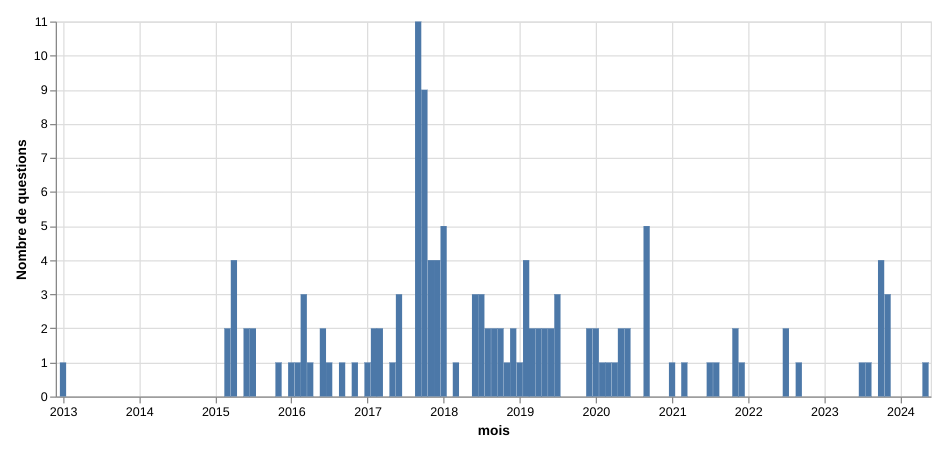
\includegraphics[width=\linewidth]{/home/thgir/Documents/travail/utbm/so03/iramuteq/img/questions_per_month}
        \caption{Nombre de questions mentionnant le glyphosate par mois}
        \label{fig:questions_per_month}
    \end{figure}

    En se basant sur le graphique~\ref{fig:questions_per_month},
    on s'aperçoit d'une très forte concentration du nombre de questions
    entre octobre 2017 et février 2018, ce qui correspond au plus fort
    du débat sur le glyphosate.
    Cette période a été marquée par de vifs débats au niveau européen,
    sur fond de nouvelles estimations sur ses dangers
    et de manipulation des études scientifiques et des évaluations officielles
    par Monsanto\cite{glyphosate-monsanto}.

    Une deuxième période de questions, bien que moins marquée,
    se situe entre juin 2018 et août 2019.
    Cette période a été marquée par le projet de loi Agriculture
    et Alimentation, dite loi EGalim
    (établissant le plan d'arrêt de l'usage du glyphosate,
    mais sans fixer de date précise
    et en établissant des dérogations\cite{loi-alimentation}),
    ainsi que par la publication du rapport de l'Agence Nationale de Sécurité Sanitaire
    de l'Alimentation, de l'Environnement et du Travail (ANSES),
    établissant les dangers liés à la présence
    de glyphosate dans les produits intimes\cite{anses-glyphosate}.


    \begin{figure}[h]
        \centering

        \begin{tabular}{l>{\centering}m{5em}>{\centering}m{5em}>{\centering}m{5em}}
            \toprule
            Orientation politique & nombre de questions & pourcentage du corpus & contribution relative (15\textsuperscript{ème} législature) \tabularnewline
            \midrule
            extrême-droite        & 8                   & 6,20\%        & 4,85 \tabularnewline
            droite                & 32                  & 24,81\%       & 1,16 \tabularnewline
            centre                & 42                  & 32,56\%       & 0,45 \tabularnewline
            gauche                & 47                  & 36,43\%       & 2,16 \tabularnewline
            \bottomrule
        \end{tabular}
        \caption{Contribution au corpus, par bloc politique}
        \label{fig:questions-par-bloc}
    \end{figure}

    Afin de se rendre compte de la contribution de chaque bloc politique au corpus,
    la figure~\ref{fig:questions-par-bloc} montre le nombre
    de questions au gouvernement issus de chacun d'entre eux,
    avec le pourcentage que celui-ci représente par rapport au nombre
    de questions total.
    Il faut toutefois se rappeler que si la contribution
    au corpus varie selon les blocs politiques,
    leur représentation proportionnelle aussi.
    La majorité des questions a été posée durant la XV\textsuperscript{ème}
    législature.
    Or, durant celle-ci, l'extrême-droite occupait 10 sièges sur 577,
    soit 5,7\% du total.

    C'est pourquoi la contribution relative lors de la 15\textsuperscript{ème}
    législature est également renseignée.
    Celle-ci est obtenue en faisant le rapport entre la proportion
    de questions posées durant cette législature et la proportion
    de députés du bloc dans le même temps, soit la formule suivante :

    $$
    \text{Contribution relative} = \frac{\text{\% de questions dans le corpus}}{\text{\% de députés}}
    $$

    Un résultat proche de 1 signifie une contribution au corpus
    proportionnelle au nombre de député, un résultat supérieur
    à 1 une contribution relative plus importante,
    et un résultat inférieur à 1 une contribution relative plus faible.

    Ce nombre est toujours à prendre avec des pincettes,
    puisqu'il ne représente que la XV\textsuperscript{ème}
    législature et qu'une faible contribution absolue
    au corpus peut tout de même être associée à une
    forte contribution relative :
    durant cette législature, l'extrême-droite a posé une seule
    question mentionnant le glyphosate, ce qui reste assez pour
    leur attribuer une grande contribution relative à leur poids
    dans l'hémicycle.
    Il permet toutefois de faire une première estimation
    de l'importance que chaque bloc porte au sujet.


    \section{Analyse factorielle des correspondances}\label{sec:analyse-factorielle-des-correspondances}

    Une fois effectuée cette analyse préliminaire de notre
    corpus, de ses liens avec l'actualité nationale
    et de la contribution des différents blocs politiques,
    il nous faut chercher quels sont les éléments de langage
    structurant la pensée de chaque bloc sur la question
    du glyphosate.

    Une AFC avec le logiciel IRaMuTeQ permet de mettre en avant
    les corrélations entre les groupes d'éléments de langage,
    en fonction de la modalité \textit{Orientation politique}.

    La figure~\ref{fig:afc-modalites} montre une séparation
    claire des quatre blocs politiques selon
    deux variables portant la quasi-totalité de l'information
    (51,7\% et 26,9\%, soit 78,6\% de l'information au total).
    La première variable oppose surtout la gauche et l'extrême-droite
    à la droite et au centre, tandis que la deuxième oppose
    surtout le centre et la gauche à la droite et à l'extrême-droite.

    Sans étonnement, le mot glyphosate, commun à la totalité
    des textes, se retrouve au centre, de même que le mot ministre.

    \begin{figure}[p]
        \centering
        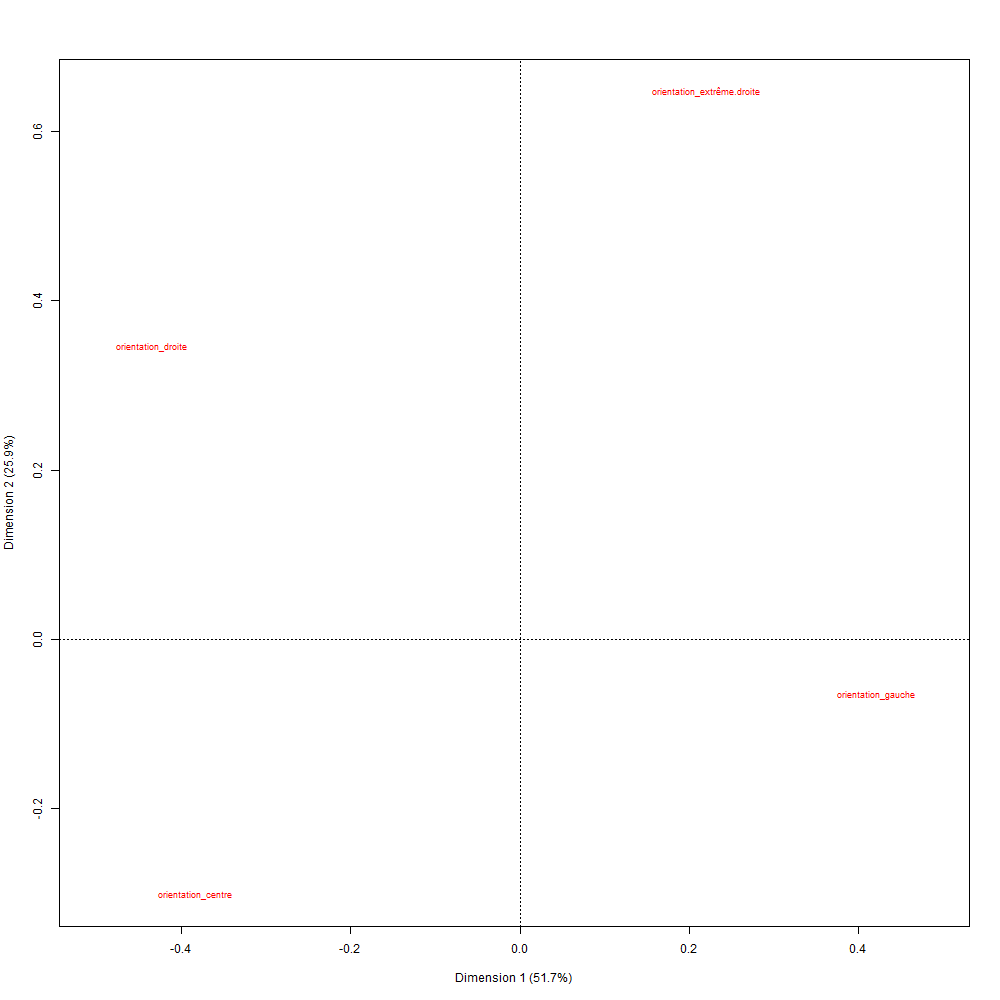
\includegraphics[width=\linewidth]{afcf_col}
        \caption{
            Analyse factorielle des correspondances du corpus en fonction
            de la variable \textit{bloc politique} - Répartition des modalités
        }
        \label{fig:afc-modalites}
    \end{figure}
    \begin{figure}[p]
        \centering
        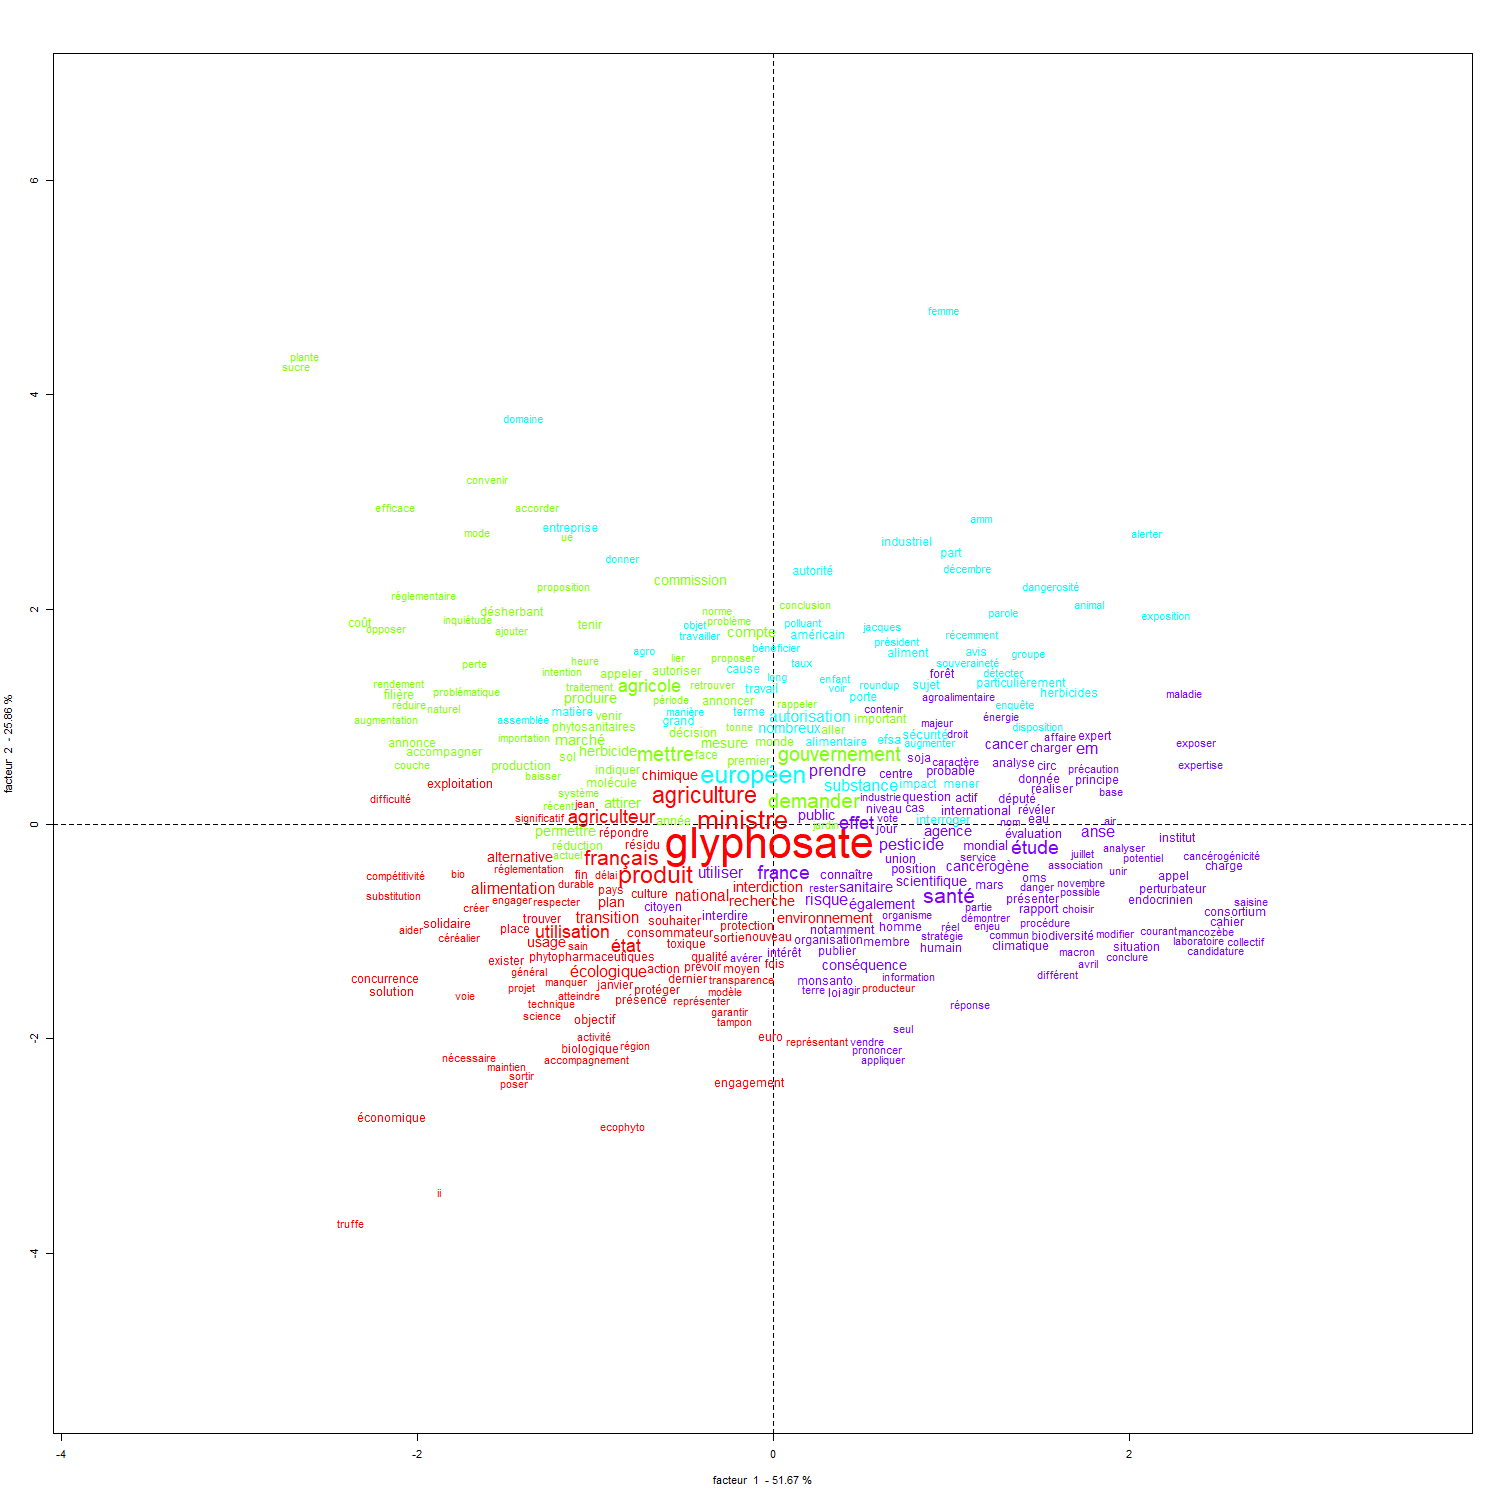
\includegraphics[width=\linewidth]{graph_afc_1}
        \caption{
            Analyse factorielle des correspondances du corpus en fonction de la variable \textit{bloc politique}
            - Répartition lexicale
        }
        \label{fig:afc-lexical}
    \end{figure}

    \subsection{La santé contre la compétitivité}\label{subsec:la-sante-contre-la-competitivite}

    Lexicalement, la première variable semble opposer deux
    visions antagonistes : la première s'appuie sur
    les études menées sur les dangers du glyphosate pour demander
    des mesures pour l'interdire, ou au moins le restreindre
    fermement ; la deuxième invoque la nécessité
    de s'adapter à la concurrence internationale et la comparaison
    aux autres pays de l'UE, pour justifier une politique
    plus incitative que restrictive.

    La première vision se trouve sur la partie droite
    du graphique, du côté des groupes de gauche et d'extrême-droite.
    On peut y retrouver de nombreuses références aux agences
    de contrôle et de recherche (ANSES, EFSA, OMS, etc.).
    l'ANSES, tout particulièrement
    est mentionnée dans 25\% des questions de l'extrême-droite
    et 23\% des questions de la gauche, contre 12,5\%
    pour la droite et 7\% sur le centre.
    Le mot « étude » se distingue également, tout en restant
    proche du mot « ANSES », de même que le mot « scientifique »,
    que l'on peut retrouver fortement corrélé à « santé ».
    Cet appui sur des études sanitaires s'intègre dans une analyse
    des effets (le mot « effet » ressort d'ailleurs de manière assez distincte)
    du glyphosate.

    Cependant, la gauche et l'extrême-droite n'abordent pas
    cette question sous le même angle.
    La gauche se concentre en effet plus sur la santé,
    la biodiversité et le climat.
    Les mots « conséquence », « climatique », « cancérogène »,
    « perturbateur endocrinien » et « biodiversité »
    sont fortement liés à la gauche, ce qui témoigne
    probablement d'une attention particulière à la
    sécurité sanitaire et écologique globale
    ainsi qu'à la protection des populations.
    De son côté l'extrême-droite,
    sans totalement ignorer la question sanitaire, a un discours
    beaucoup moins clair.
    Le mot « cancer » se retrouve ainsi à la frontière entre la gauche
    et l'extrême-droite, de même que les mots « maladie »,
    « impact » et « agro-alimentaire », ce qui semble indiquer
    certaines préoccupations communes avec la gauche.
    Cependant, en dehors de ces quelques mots frontière,
    aucun schéma de pensée clair ne semble se dessiner.
    Cela peut s'expliquer à la fois par la faible quantité
    de textes issus de l'extrême-droite dans notre corpus,
    ainsi que par une incohérence idéologique sur la question ;
    nous reviendrons plus tard sur ce deuxième point.

    La seconde vision, qui se trouve sur la partie gauche
    et qui rapproche le centre et la droite,
    oppose au souci sanitaire susmentionné la question
    de la compétitivité de l'agriculture.
    Dans le bloc politique central, on retrouve ainsi,
    très groupés, les mots « compétitivité »,
    « substitution », « concurrence » et « solution »,
    ce qui traduit un changement de paradigme :
    la sortie du glyphosate ne se fait plus par la réglementation
    de manière planifiée et dans des délais fixés,
    mais par le développement d'alternatives techniques
    et économiques et un accompagnement de cette transition.
    Les mots « transition », « alternative », « agriculteur »
    et « écologique » sont ainsi très présents
    dans le bloc politique du centre.
    Le centre, bien que montrant une volonté de sortir
    du glyphosate, se distingue de la gauche par
    la place primordiale laissée à la concurrence
    et à la compétitivité, ainsi que par une vision techno-solutionniste,
    qui s'inscrit dans un récit post-nature de l'anthropocène.

    Si la droite semble partager quelques uns de ces éléments de langage
    (« agriculteur », « réduction » et « alternative » se trouvent
    à la frontière entre les deux),
    elle ne semble pas articuler son discours autour
    de concepts précis ;
    en-dehors d'« agricole » et des mots-frontière,
    aucun ne ressort particulièrement.
    L'absence de tout mot relevant du champ lexical de la santé
    et de celui de l'interdiction (au contraire, on
    remarque une forte proximité des mots « agricole »,
    « autoriser » et « produire »)
    laisse même douter de toute volonté de sortir du glyphosate.
    La droite apparait ainsi comme partageant la vision
    concurrentiel du centre, mais sous un angle bien plus conservateur,
    qui ne prévoit pas de sortie du glyphosate.

    Trois pensées principales se retrouvent donc dans ce corpus :

    \begin{itemize}
        \item Une vision conservatrice et concurrentielle, portée
        par la droite,
        \item Une vision libérale et techno-solutionniste, portée par le centre,
        envisageant une sortie du glyphosate à travers la recherche d'alternatives
        \item Une vision centrée sur les enjeux sanitaires et écologiques, portée
        par la gauche, se préoccupant des impacts du glyphosate
    \end{itemize}


    \subsection{Le cas de l'extrême-droite}\label{subsec:le-cas-de-l'extreme-droite}

    Un discours précis ne se dessine pas pour l'extrême-droite,
    malgré quelques points idéologiques communs avec la gauche
    et certaines préoccupations d'ordre sanitaire.
    Un examen texte par texte peut nous permettre d'y voir plus clair.
    En raison de la faible contribution de l'extrême-droite
    au corpus dans l'absolu (huit textes seulement), cette analyse en détail est en
    effet plus pertinente qu'une simple analyse quantitative.

    En raison des orientations du Front National en ce qui concerne
    l'écologie, on pourrait s'attendre à une ligne favorable à l'usage
    des glyphosates transparaissant clairement dans les questions
    au gouvernement.
    Les députés Front National ont ainsi tous voté entre faveur
    de l'extension à la culture des betteraves des exemptions
    d'interdiction d'usage du glyphosate en 2020~\cite{vote-glyphosate} ;
    plus proche de nous, ils ont également porté des amendements
    visant à rendre ineffectif de fait l'interdiction du glyphosate
    dans l'agriculture~\cite{amendement-glyphosate}.

    Et pourtant, les mots employés par l'extrême-droite sont
    mélangés en grande partie avec ceux de la gauche et avec
    ceux de la droite et semblent porter un sens
    contraire à celui des votes réels de l'extrême-droite.

    En réalité, il apparait que la moitié des questions de l'extrême-droite
    du corpus ont été émises par M. Jacques Bompard, un des membres fondateurs
    du FN, ayant quitté le parti en 2005 pour rejoindre le MPF de Philippe
    de Villiers, puis ayant fondé son propre parti en 2010.
    Il s'agit donc bien d'un député d'extrême-droite, mais non-encarté,
    ce qui peut expliquer des divergences avec le Front National.
    De plus, ses questions ont toutes été posées durant la XIV\textsuperscript{ème}
    législature (étant donné qu'il a démissionné de sa fonction de député en août
    2017 en raison de la législation sur le cumul des mandats),
    c'est-à-dire avant la principale vague de questions, fin 2017.

    Dans ses questions, il témoigne d'un souci de défense des agences de
    recherche et de contrôle contre le groupe Monsanto,
    notamment dans celle du 13 juin 2017~\cite{bombard-question}.
    Ces références aux agences reviennent dans la plupart de ses questions :
    CIRC~\cite{bombard-question}, EFSA, ECHA, OMS~\cite{bombard-question-2},
    ANSES~\cite{bombard-question-3}\ldots
    Il s'appuie sur les études de ces organismes pour établir
    les effets sanitaires néfastes du glyphosate, notamment
    ses effets cancérogènes probables.

    Cependant, cette pensée ne s'intègre pas dans un cadre écologique
    et sanitaire global, comme on peut le voir à gauche,
    mais plus dans une défense des agriculteurs,
    dont l'idéalisation rappelle par moment le « retour à la terre »
    du régime de Vichy.
    Ainsi, dans sa question du 1er novembre 2016~\cite{bombard-question-3} :

    \begin{quotation}
        « Les agriculteurs doivent retrouver la nature originelle de leur travail.
        Un labeur noble, responsable de la santé des Français et de la beauté des territoires.\ »
    \end{quotation}

    Nous avons donc ici à faire à un discours dont on pourrait
    interroger la portée confusionniste
    et qui, en raison de son poids important dans sa modalité
    du corpus, brouille notre analyse quant à la position de l'extrême-droite
    sur la question du glyphosate.

    Si cette opposition au glyphosate peut se retrouver dans une autre
    question, celle de Stéphane Rambaud du 26 juillet 2022~\cite{rambaud-question},
    c'est encore une fois motivé principalement par la question
    de la défense des agriculteurs (il y est ici question de la filière apicole).

    Toutes les autres questions justifient de la même manière
    leur propos par la défense des agriculteurs, mais en prenant
    une posture clairement opposée à l'interdiction du glyphosate.

    Ainsi, la seule base idéologique constante identifiée
    au sein de l'extrême-droite vis-à-vis du glyphosate n'est pas liée
    au glyphosate en lui-même, mais aux agriculteurs,
    et à leur défense réelle ou supposée, contre des grands organismes
    à la désignation variante (Monsanto, l'UE, la concurrence ukrainienne).
    La volonté d'interdire ou non le glyphosate varie ainsi
    dans le temps et les sous-groupes politiques constituant l'extrême-droite.
    Aujourd'hui, la tendance semble être à demander la levée
    de son interdiction.

    \section{Limites de l'analyse}\label{sec:limites-de-l'analyse}

    Si notre analyse a permis de mettre en avant certains
    marqueurs idéologiques entre les blocs politiques,
    elle est néanmoins marqué par certains défauts qui limitent sa portée.

    Principalement, la taille relativement faible du corpus de texte :
    avec 133 questions de 289 mots en moyenne, répartis en quatre modalités,
    la masse de données est trop faible pour une étude quantitative
    approfondie.
    Le croisement avec des sources secondaires (articles de presse,
    autres documents de l'Assemblée nationale) permet
    en partie de pallier ce problème,
    mais il n'en reste pas moins que l'AFC en elle-même
    porte trop peu d'information et que les résultats peuvent
    être influencés très fortement par les questions
    de quelques députés, ce qui nuit à notre objectif,
    qui était d'établir les idées structurantes des blocs
    politiques en tant que formations collectives.

    Le flou idéologique de la droite et de l'extrême-droite,
    combiné à cette faible taille du corpus, a accentué
    cet effet et rendu l'AFC beaucoup plus confuse qu'elle n'aurait
    dû l'être.

    \section{Conclusion}\label{sec:conclusion}

    Au travers de notre étude, nous avons pu établir
    les principaux moments de la question du glyphosate,
    c'est-à-dire les périodes octobre 2017--février 2018 et
    juin 2018--août 2019.

    Nous avons pu également, grâce à l'AFC, croisée avec
    d'autres données parlementaires et combinée
    avec l'analyse au cas-par-cas de certains des textes,
    établir certaines idées structurantes de la position
    des différents blocs sur le glyphosate :
    on y distingue une gauche portée sur les questions
    sanitaires et écologiques, poussant l'interdiction
    du glyphosate, une droite à la vision conservatrice et concurrentielle,
    opposée à son interdiction, un centre libéral et techno-solutionniste,
    favorable à une fin du glyphosate sans planification précise
    et conditionnée par l'émergence d'alternatives, et enfin une extrême-droite
    ruraliste, à l'opinion d'abord floue, avant de se ranger du côté
    de l'opposition à l'interdiction du glyphosate.

    Afin d'aller plus loin, nous pourrions étendre notre étude,
    afin d'y intégrer les avis sur d'autres produits phytosanitaires
    controversés, tels que les néonicotinoïdes, évoqués au début de ce rapport.


    \newpage


    \listoffigures

    \newpage

    \bibliography{main} % Entries are in the refs.bib file
    \bibliographystyle{plain}

\end{document}
